\documentclass[10pt,twocolumn,letterpaper]{article}

\usepackage{ltxgrid}
\usepackage{listings}
\usepackage{iccv}
\usepackage{times}
\usepackage{epsfig}
\usepackage{graphicx}
\usepackage{amsmath}
\usepackage{amssymb}
\usepackage{multirow}
\usepackage{microtype}
\usepackage{enumitem}
\setlist{nolistsep}
\usepackage{url}

\lstset{ 
        language=Matlab,                                % choose the language of the code
%       basicstyle=10pt,                                % the size of the fonts that are used for the code
        numbers=left,                                   % where to put the line-numbers
        numberstyle=\footnotesize,                      % the size of the fonts that are used for the line-numbers
        stepnumber=1,                                           % the step between two line-numbers. If it's 1 each line will be numbered
        numbersep=5pt,                                  % how far the line-numbers are from the code
%       backgroundcolor=\color{white},          % choose the background color. You must add \usepackage{color}
        showspaces=false,                               % show spaces adding particular underscores
        showstringspaces=false,                         % underline spaces within strings
        showtabs=false,                                         % show tabs within strings adding particular underscores
%       frame=single,                                           % adds a frame around the code
%       tabsize=2,                                              % sets default tabsize to 2 spaces
%       captionpos=b,                                           % sets the caption-position to bottom
        breaklines=true,                                        % sets automatic line breaking
        breakatwhitespace=false,                        % sets if automatic breaks should only happen at whitespace
        escapeinside={\%*}{*)}                          % if you want to add a comment within your code
}



% Include other packages here, before hyperref.

% If you comment hyperref and then uncomment it, you should delete
% egpaper.aux before re-running latex.  (Or just hit 'q' on the first latex
% run, let it finish, and you should be clear).
\usepackage[breaklinks=true,bookmarks=false,hidelinks]{hyperref}

\iccvfinalcopy % *** Uncomment this line for the final submission

\def\iccvPaperID{614} % *** Enter the ICCV Paper ID here
\def\httilde{\mbox{\tt\raisebox{-.5ex}{\symbol{126}}}}

% Pages are numbered in submission mode, and unnumbered in camera-ready
%\ificcvfinal\pagestyle{empty}\fi
\setcounter{page}{1} % {4321}

\begin{document}

%%%%%%%%% TITLE

% \title{The best title of all time \kevin{think up best title of all time}}

\title{A Kalman Filter Performance Analysis}

\author{Kevin Matzen}

\maketitle
%\thispagestyle{empty}
\twocolumngrid

\begin{abstract}
We evaluate the performance of several filtering algorithms for pose estimation of a mobile GPS receiver.  Often, model parameters such as process and measurement noise covariances are not known a priori, so engineers must hand-tune these per application and then evaluate them to ensure quality and stability.  We found that a simple time-varying Kalman filter with an empirically derived measurement noise covariance and a static, hand-tuned process noise covariance performs quite well for our mobile datasets, is simple to implement, and is easy to tune.  We perform both qualitative pose evaluations using maps as well as quantitative stability and statistical hypothesis tests to validate the model of our system.
\end{abstract}

\section{Introduction}\label{sec:intro}
In real world systems contaminated with noise, it's often desirable to fuse measurements and predictions from multiple sources in order to leverage orthogonal information.  One widely used filter is the Kalman filter.  A Kalman filter is applicable when the states are linear with respect to both some physical process model as well as some measurements and both the process and measurements are contaminated by some Gaussian white noise.

In particular, let $x_k$ be the state at epoch $k$, $A$ be the process matrix that predicts $x_{k+1}$ given $x_k$, $z_k$ be the measurements, $R_k$ be the measurement noise covariance matrix, and $Q_k$ be the process noise covariance matrix.  Additionally, let $C$ be a matrix that maps states to measurements and let $G$ be a matrix that maps the process noise covariance matrix to the state space.  The family of systems that take no control input and that can be modeled by a Kalman filter is described by the following equations:\\
\begin{equation}
\begin{aligned}
x_{k} &=& A x_{k-1} + G q_{k}\\
z_{k} &=& C x_{k-1} + r_{k}\\
q_{k} &\sim& N(0, Q_k)\\
r_{k} &\sim& N(0, R_k)\\
E[qr^T] &=& 0
\end{aligned}
\end{equation}

The Kalman filtering algorithm can be decomposed into two steps.  First, the process model is used to compute an a priori prediction distribution, $N(\hat{x}_{k|k-1}$, $P_{k|k-1})$, called the prediction step.  Then, the measurements are fused to produce an improved a posteriori estimate distribution, $N(\hat{x}_{k|k}$, $P_{k|k})$, during the update step.  Assuming the process is modeled correctly and the noise covariance matrices are correct, then the Kalman filter provides the optimal estimate of the state.

The Kalman filter equations are as follows:\\
{\bf Prediction:}
\begin{equation}
\begin{aligned}
\hat{x}_{k|k-1} &=& A \hat{x}_{k-1|k-1}\\
P_{k|k-1} &=& A P_{k-1|k-1} A^T + Q_k
\end{aligned}
\end{equation}
{\bf Update:}
\begin{equation}
\begin{aligned}
\tilde{y}_k &=& z_k - C \hat{x}_{k|k-1}\\
S_k &=& C P_{k|k-1} C^T + R_k\\
K_k &=& P_{k|k-1} C^T S_k^{-1}\\
\hat{x}_{k|k} &=& \hat{x}_{k|k-1} + K_k \tilde{y}_k\\
P_{k|k} &=& (I - K_k C) P_{k|k-1}
\end{aligned}
\end{equation}
where
\begin{equation}
\begin{aligned}
E[x_k - \hat{x}_{k|k}] &=& 0\\
E[(x_k - \hat{x}_{k|k})(x_k - \hat{x}_{k|k})^T] &=& P_{k|k}\\
E[x_k - \hat{x}_{k|k-1}] &=& 0\\
E[(x_k - \hat{x}_{k|k-1})(x_k - \hat{x}_{k|k-1})^T] &=& P_{k|k-1}\\
E[\tilde{y}_k] &=& 0\\
E[\tilde{y}_k\tilde{y}_k^T] &=& S_k\\
\end{aligned}
\end{equation}
Briefly, the prediction step propagates the state forward using the process model and convolves it with the process noise model, $N(A\hat{x}_{k-1|k-1}, E[(Ap_{k-1})(Ap_{k-1})^T]) \ast N(0, Q_k)$ where $p_{k-1} \sim P_{k-1|k-1}$.
 The update step uses the definitions of $P_{k|k}$, $\hat{x}_{k|k}$, $\tilde{y}_k$, and $z_k$, and a series of substitutions to arrive at the optimal Kalman gain.

While the Kalman filter offers optimality when the underlying assumptions hold, it is often the case that they do not hold.  Noise is often correlated, biases are often present, the process model is often not expressive of the true process, and noise covariances are often unknown.  Indeed, biases in GPS measurements are present in the form of multipath error and differences between true atmospheric delays and approximate atmospheric models.  It is very easy to qualitatively validate the design of a filter, but more importantly, it's desireable to understand how well we've modeled the system, that is, do any of the underlying assumptions actually hold and if so, how confident are we that they hold?

We explore the use of statistical hypothesis tests to help drive the tuning of our Kalman fitler parameters.  Section~\ref{sec:theory} details the high-level design of our filter and describes a test to determine whether our filter is consistent, that is, $\tilde{y}_k \sim N(0,S_k)$.  We also briefly explore extending the filter to include per-satellite biases in the filter state and show that we can decrease uncertainty while maintaining consistency.  Section~\ref{sec:experiments} describes a series of experiments performed on both stationary receiver data, where we can emperically derive the measurement covariance matrix and the process model intuitively holds well, as well as data from a moving receiver where assumptions regarding the process model are frequently broken.  We conclude with Section~\ref{sec:conclusion} describing a few ideas for reducing biases and better modeling the process.

\section{Theory}\label{sec:theory}
First we describe the particular system we intend to model and then we describe specific statistical hypothesis tests that we applied to validate the model.

\subsection{Model}
The system model used in this work is similar to the one presented in~\cite{course}.  This system has 11 core states, position, velocity, acceleration, clock offset, and clock rate offset and 8 are realized as measurements, namely, position, velocity, clock offset, and clock rate offset.
\begin{equation}
x_k = \left[
\begin{array}{c}
\vec{x}_k\\
\vec{\dot{x}}_k\\
\vec{\ddot{x}}_k\\
c\delta_{Rk}\\
c\dot{\delta}_{Rk}\\
\end{array}
\right],
z_k = \left[
\begin{array}{c}
\vec{x}_k\\
\vec{\dot{x}}_k\\
c\delta_{Rk}\\
c\dot{\delta}_{Rk}\\
\end{array}
\right]
\end{equation}
The state transition matrix used to model the system dynamic is a constant acceleration model described by
\begin{equation}
A_k = \left[
\begin{array}{ccccc}
I_{3\times3} & \delta_{T_{Rk}}I_{3\times3} & \frac{1}{2}\delta_{T_{Rk}}^2I_{3\times3} & 0 & 0\\
0 & I_{3\times3} & \delta_{T_{Rk}}I_{3\times3} & 0 & 0\\
0 & 0 & I_{3\times3} & 0 & 0\\
0 & 0 & 0 & 1 & \delta_{T_{Rk}}\\
0 & 0 & 0 & 0 & 1\\
\end{array}
\right]
\end{equation}
where
\[\delta_{T_{Rk}} = \frac{t_{Rk+1} - t_{Rk}}{1 + \dot{\delta}_{Rk}}\]

For this work, the process covariance matrix is simply $Q_k = \alpha_kI_{4\times4}$ and the matrix used to map this into the state space is
\begin{equation}
G = \left[
\begin{array}{cc}
0 & 0\\
0 & 0\\
0 & 0\\
0 & 0\\
0 & 0\\
0 & 0\\
I_{3\times3} & 0\\
0 & 0\\
0 & 1\\
\end{array}
\right]
\end{equation}

In order to best accomadate the geometric receiver-satellite configuration, the measurement covariance matrix is designed to consider the position and velocity DOP matrices, $Q_P$ and $Q_V$ for the position and velocity solutions respectively.  An additional assumption is that this measurement uncertainty can be accurately modeled using global $\sigma_{PR}$ and $\sigma_{D}$.  
Let 
\begin{equation}
\sigma_{PR}^2Q_P = 
\left[
\begin{array}{cc}
\Sigma_x & \vec{\sigma}_{x,t}^T\\
\vec{\sigma}_{x,t} & \sigma_t
\end{array}
\right],
(\lambda_{L1}\sigma_D)^2Q_V = \left[
\begin{array}{cc}
\Sigma_{\dot{x}} & \vec{\sigma}_{\dot{x},\dot{t}}^T\\
\vec{\sigma}_{\dot{x},
\dot{t}} & \sigma_{\dot{t}}\\
\end{array}
\right]
\end{equation}
\begin{equation}
R_k = \left[
\begin{array}{cccc}
\Sigma_x & 0 & \vec{\sigma}_{x,t}^T & 0\\
0 & \Sigma_{\dot{x}} & 0 & \vec{\sigma}_{\dot{x},\dot{t}}^T\\
\vec{\sigma}_{x,t} & 0 & \sigma_t & 0\\
0 & \vec{\sigma}_{\dot{x},\dot{t}} & 0& \sigma_{\dot{t}}\\
\end{array}
\right]
\end{equation}
The matrix used to map measurements into the state space is
\begin{equation}
C = \left[
\begin{array}{cccc}
I_{3\times3} & 0 & 0 & 0\\
0 & I_{3\times3} & 0 & 0\\
0 & 0 & 0 & 0\\
0 & 0 & 0 & 0\\
0 & 0 & 0 & 0\\
0 & 0 & 1 & 0\\
0 & 0 & 0 & 1\\
\end{array}
\right]
\end{equation}

One thing that is immediately clear from this formulation is that while the Kalman filter considers measurement noise, it does so under the assumption that it is unbiased.  As stated earlier, there are several factors that lead to error in GPS observables, notably multipath and atmospheric mis-modeling.  These errors are often slowly varying, so in a small time window, they can be modeled as measurement bias.  We propose a simple extention to the suggested model by extending the state to include the core state plus per-satellite pseudorange and doppler shift biases.  These biases are introduced into the system as measurements via the residuals from the navigation and velocity solutions.
\begin{equation}
x_{bk} = \left[
\begin{array}{c}
x_k\\
\vec{b}_{PRk}\\
\vec{b}_{Dk}\\
\end{array}
\right],
z_{bk} = \left[
\begin{array}{c}
z_k\\
\vec{b}_{PRk}\\
\vec{b}_{Dk}\\
\end{array}
\right],
\end{equation}
Similary, the process and measurement covariance matrices are extended using hand-tuned parameters:
\begin{equation}
R_{bk} = \left[
\begin{array}{ccc}
R_k & 0 & 0\\
0 & \beta I_{32\times32} & 0\\
0 & 0 & \gamma I_{32\times32}\\
\end{array}
\right]
\end{equation}
\[Q_b = \alpha_k I_{75\times75}\]
Since only a subset of satellite biases are observable at any given epoch, the matrix $C$ is now time varying and has entries for unobserved satellites set to $0$.

\subsection{Hypothesis Tests}
Based on the assumptions underlying the Kalman filter one might wish to answer the following questions:
\begin{enumerate}
\item Are my filter's innovations white?
\item Is my estimator consistent?
\item Might a particular measurement destroy the integrity of my filter?
\end{enumerate}
Each of these questions can be answered with well-established hypothesis tests.

\medskip
\noindent{\bf Innovation Whiteness} In practice, this can be a difficult test to pass since it's clear that errors between measurements from GPS data are slowly varying and correlated.  However, it is something to test for to validate that claim.  There are many possible tests for whiteness of multivariate random variables.  We present the multivariate generalization of the Ljung-Box test.

Our hypothesis test is defined as follows:\\
$H_0$: Innovations are independently distributed.\\
$H_1$: Innovations are not independently distributed.\\
For a maximum lag $h$, innovation dimensionality $K$, and track length $T$,
\begin{eqnarray*}
C_i &=& \frac{1}{T}\sum_{t=i+1}^T\tilde{y}_t\tilde{y}_{t-i}^T\\
Q &=& T(T+2)\sum_{j=1}^h \frac{tr\{C_j^T C_0^{-1} C_j C_0^{-1}\}}{T-j}\\
\end{eqnarray*}
where $\tilde{y}_t$ is the innovation at epoch $t$, $C_i$ the multivariate sample autocorrelation at lag $i$, and $Q$ is our test statistic.
According to a one-tailed test, if $Q > \chi^2_{1-\alpha,K^2h}$ where $\chi^2_{x,v}$ is the CDF of the $\chi^2$ distribution with $v$ degrees of freedom at $x$, then we reject $H_0$.

\medskip
\noindent Informal Explaination - Consider a simpler statistic, the Box-Pierce test, $Q = T \sum_{j=1}^h tr\{C_j^T C_0^{-1} C_j C_0^{-1}\}$.
\begin{eqnarray*}
tr\{C_j^T C_0^{-1} C_j C_0^{-1}\} &=& \sum_{a,b}[(C_j^T C_0^{-1})^T(C_j C_0^{-1})]_{a,b}\\
 &=& \sum_{a,b}[(C_0^{-T} C_j)(C_j C_0^{-1})]_{a,b}\\
 &=& \sum_{a,b}[(C_0^{-1} C_j)(C_j C_0^{-1})]_{a,b}\\
 &=& \sum_{a,b}[C_0^{-1} C_j^2 C_0^{-1}]_{a,b}\\
\end{eqnarray*}
This is a sum of squares after the samples have been normalized from their source distributions to the unit covariance distribution.  If each element really is sampled independently from a normal distribution, then the sum of squares should be distributed according to a $\chi^2$ distribution of $h \times K^2$ degrees.

\medskip
\noindent Practical Considerations - This statistic is useful as-is for steady-state Kalman filters modeling a static receiver.  However, for the case of a time-varying Kalman filter, the distribution $N(0,S_k)$ changes with each sample time.  Therefore, it doesn't make sense to analyse the innovations as if they were sampled from the same distribution.  A workaround is to normalize each innovation to the $N(0, I)$ distribution as though they were sampled from $N(0,S_k)$.  That is, $\tilde{y}_k' = S_k^{-\frac{1}{2}} \tilde{y}_k$.

\medskip
\noindent{\bf Consistency Test} According to our original assumptions, $\tilde{y}_k \sim N(0, S_k)$.  The following hypothesis test can be used to see if our current model parameters are adequate.\\
$H_0$: Innovations are normally distributed.\\
$H_1$: Innovations are not normally distributed.\\
For innovation dimensionality $K$ and track length $T$
\begin{eqnarray*}
t_k &=& \tilde{y}_k^T S^{-1}_k \tilde{y}_k\\
\bar{\epsilon} &=& \sum_{k=1}^T t_k\\
\end{eqnarray*}
$t_k$ is often called the normalized innovations squared.  According to a two-tailed test, if $\alpha/2 > \chi^2_{\bar{\epsilon}, TK}$ or $1-\alpha < \chi^2_{\bar{\epsilon}, TK}$, then reject $H_0$.

\medskip
\noindent Practical Considurations - Since this is a two-tailed test, it gives us information about whether or not our model parameters produce a consistent filter as well as in what direction we should tune it, if necessary.  The $\tilde{y}_k^T S^{-1}_k \tilde{y}_k$ essentially rescales the innovation from it's source distribution down to $N(0,I)$, assuming $S_k$ was the correct covariance to begin with.  If $\bar{\epsilon}$ is too large, then that means $S^{-1}_k$ was too large and $S_k$ was too small.  Increasing $Q_k$ or $R_k$ will increase $S_k$.  Similarly, if $\bar{\epsilon}$ is too small, then we should decrease $Q_k$ or $R_k$.

\medskip
\noindent{\bf Failure Rejection} The same consistency test described earlier for filter validation and tuning can be applied online to the entire history of innovations.  If the measurement is deemed to make the consistency test reject $H_0$, then discard the measurement, but still propagate the predicted state forward.

\section{Experiments and Results}\label{sec:experiments}
Experiments were performed on both stationary and moving datasets.  Our \texttt{stationary} dataset is approximately 22 minutes long and was collected using the Upson Hall antenna on November 11, 2013 starting at approximately 7:39 PM EST.  Weather parameters for the neutral atmosphere corrections were obtained from wunderground.com.  Our moving datasets include those distributed on the course website.  While we evaluated our methods on all datasets, we present in this paper results for \texttt{airportloop} and \texttt{cudtrt13triphammercu}. \texttt{airportloop} offers an interesting case where most of the route is unaffected by multipath errors since tall buildings are not present.  Additionally, the weather measurements should be quite accurate, assuming they were acquired using the weather station located at the airport.  In contrast, \texttt{cudtrt13triphammercu} offers many challenging examples of line-of-sight occlusion and multipath reflections as well as long stretches of highway for the filter to recover.

We evaluate several versions of our time-varying Kalman filters, each with different turning parameters.  In addition, we also compare to results obtained by using a steady-state Kalman filter built with MATLAB's \texttt{dlqe}, and the two static filters described in~\cite{course}.  Interactive, qualitative results for all datasets can be viewed at \url{http://mae5150.kmatzen.com} until February 2014.  Many of the static filter and steady-state Kalman filter results are omitted from this paper since they largely overlap and are hard to visualize.

Our first attempt at designing the measurement covariance matrix involved using $\sigma_{PR}$ and $\sigma_D$ from \texttt{solveposvelod}.  In practice, we found two issues with these estimates, both stemming from being estimated by so few satellites at each epoch.  One is that they tend to vary quickly and the other is that they seem to produce filters that were over-confidence in the measurements.  We instead take a moving average of the estimated variances.  Then we tuned the process covariance matrix until the filter passed our consistency test.  For the moving datasets, tuning the process covariance matrix had very little impact on whether or not we could pass the consistency test, presumably due to model mismatch.  Instead, we scaled the measurement covariance up by some constant factor for the entire dataset until we could pass the test.

We applied the Ljung-Box hypothesis test to each track's innovations with many parameters, different subsets of the innovations (position only, velocity only, etc.), different subsets of the tracks, and so on.  It consistently rejected $H_0$ with $\alpha = 0.05$, that is, our innovations were correlated violating the white Gaussian noise assumption.

\begin{figure}
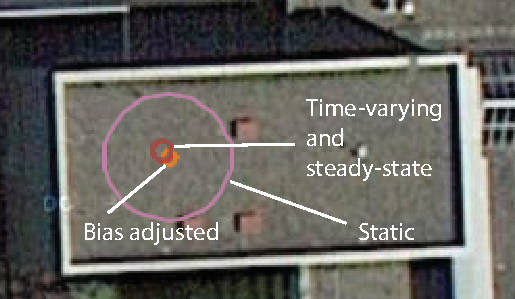
\includegraphics[width=\columnwidth]{stationary_map}
\caption{Static filter results are indicated with a large circle for clarity.  Kalman-filtered results are shown with their 99\% confidence interval ellipses projected onto the East-North plane.}
\label{fig:stationary_map} 
\end{figure}


\subsection{Stationary Receiver}
Figure~\ref{fig:stationary_map} shows the estimated position of the receiver's antenna at the end of the dataset sequence.  The consistency test was used to tune the process covariance matrix to $2\times10^{-3}I$ and the measurement covariance matrix was not rescaled.

Using the antenna's surveyed location, we computed the positional error.  Figure~\ref{fig:stationary_error} shows that during some samples, the bias adjustment model reduces error and it does not severely hinder performance at any sample time.  Our consistency test also passes when bias adjustment is enabled.  While we see some modest improvement for this stationary dataset, we do not observe appreciable benefits on any of the mobile datasets.

\begin{figure}
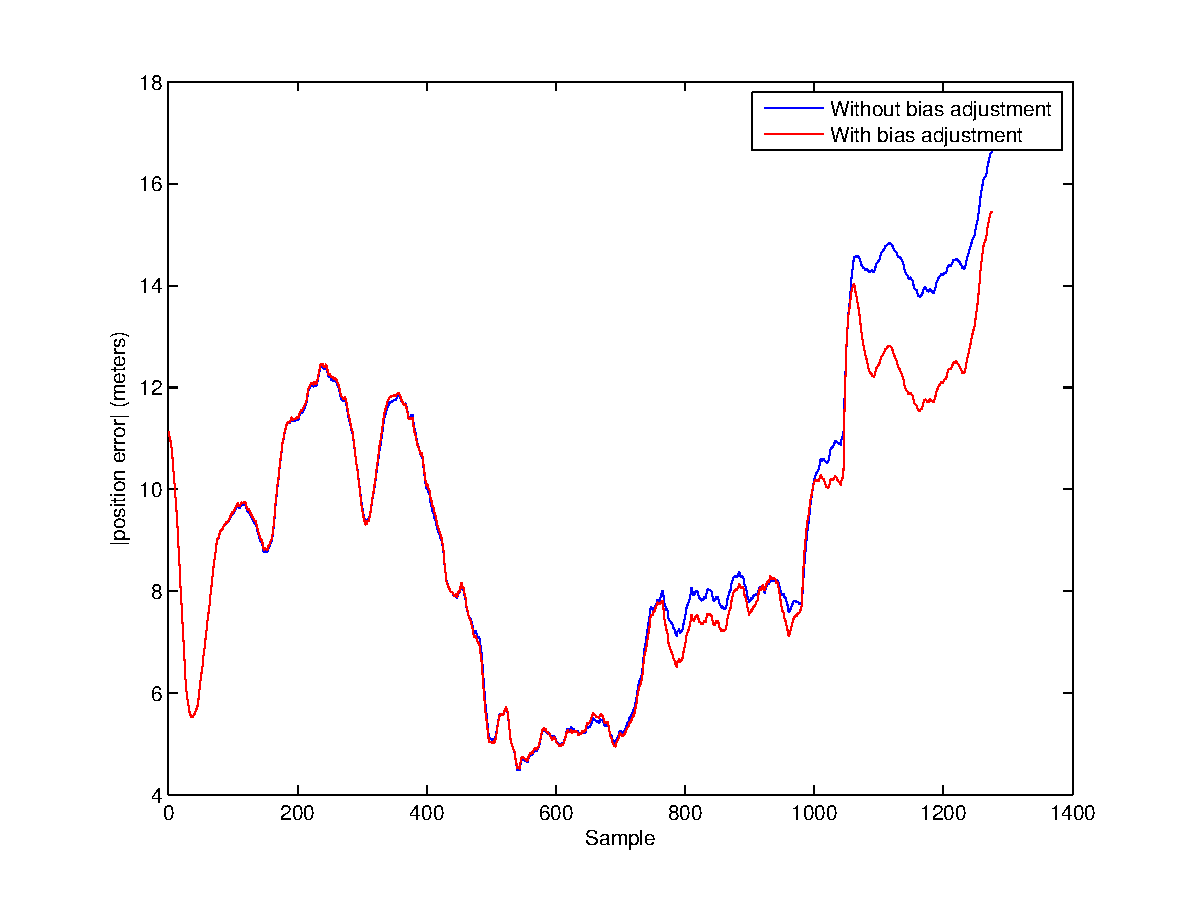
\includegraphics[width=\columnwidth]{error_stationary}
\caption{Error of estimated receiver antenna position with respect to sample time.  The bias adjusted model outperforms the base model in some cases.}
\label{fig:stationary_error}
\end{figure}

Finally, we apply the Ljung-Box test and Mardia's test to the estimated jerk of the system to check for process model mismatch for the case of the time-varying Kalman filter without bias adjustment.  The Ljung-Box test with $\alpha = 0.05$ rejects the null hypothesis test which means the jerk is correlated.  It accepts $H_0$ for Mardia's test with p-value 0.48 for the skewness statistic and 0.1242 for the kurtosis statistic.  When applied to the bias-adjusted version of the time-varying Kalman filter, Mardia's test rejects $H_0$ suggesting that we are indeed introducing a new systematic bias.

Figure~\ref{fig:nis_stationary} shows how the normalized innovation squared statistic, $t_k$ changes over time.  The green lines indicate the test bounds for a 99\% confidence interval and the blue line indicates the test value.  These normalized innovation squared values were fairly consistent, so it seems likely that this is a good way to tune the filter parameters and expect it to generalize well.

\begin{figure}
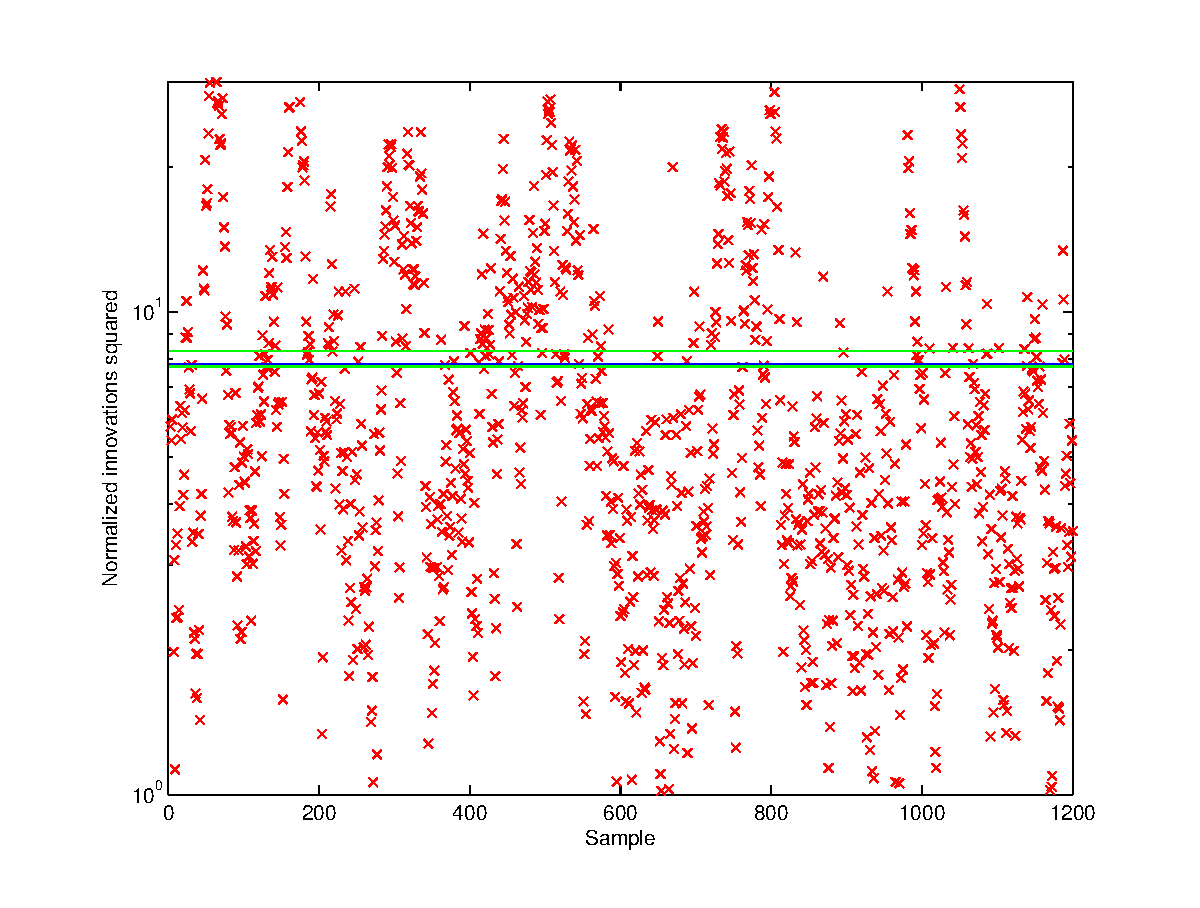
\includegraphics[width=\columnwidth]{nis_stationary}
\caption{Normalized innovation squared values for the \texttt{stationary} dataset.  The green lines represent the test bounds and the blue line is the test statistic.}
\label{fig:nis_stationary}
\end{figure}



\subsection{Airport Dataset}
Figure~\ref{fig:airportloop_map} shows the estimated trajectory of the vehicle using our time-varying Kalman filter.  This was estimated using a process covariance matrix of $Q = 10I$ and a measurement covariance matrix scaled by $3.5$ in order to pass the consistency test.  This is a very easy dataset.  Figure~\ref{fig:airportloop_map_bad} illustrates what happens if we do not scale the measurement covariance matrix to ensure a consistent filter.

\begin{figure}[!bthp]
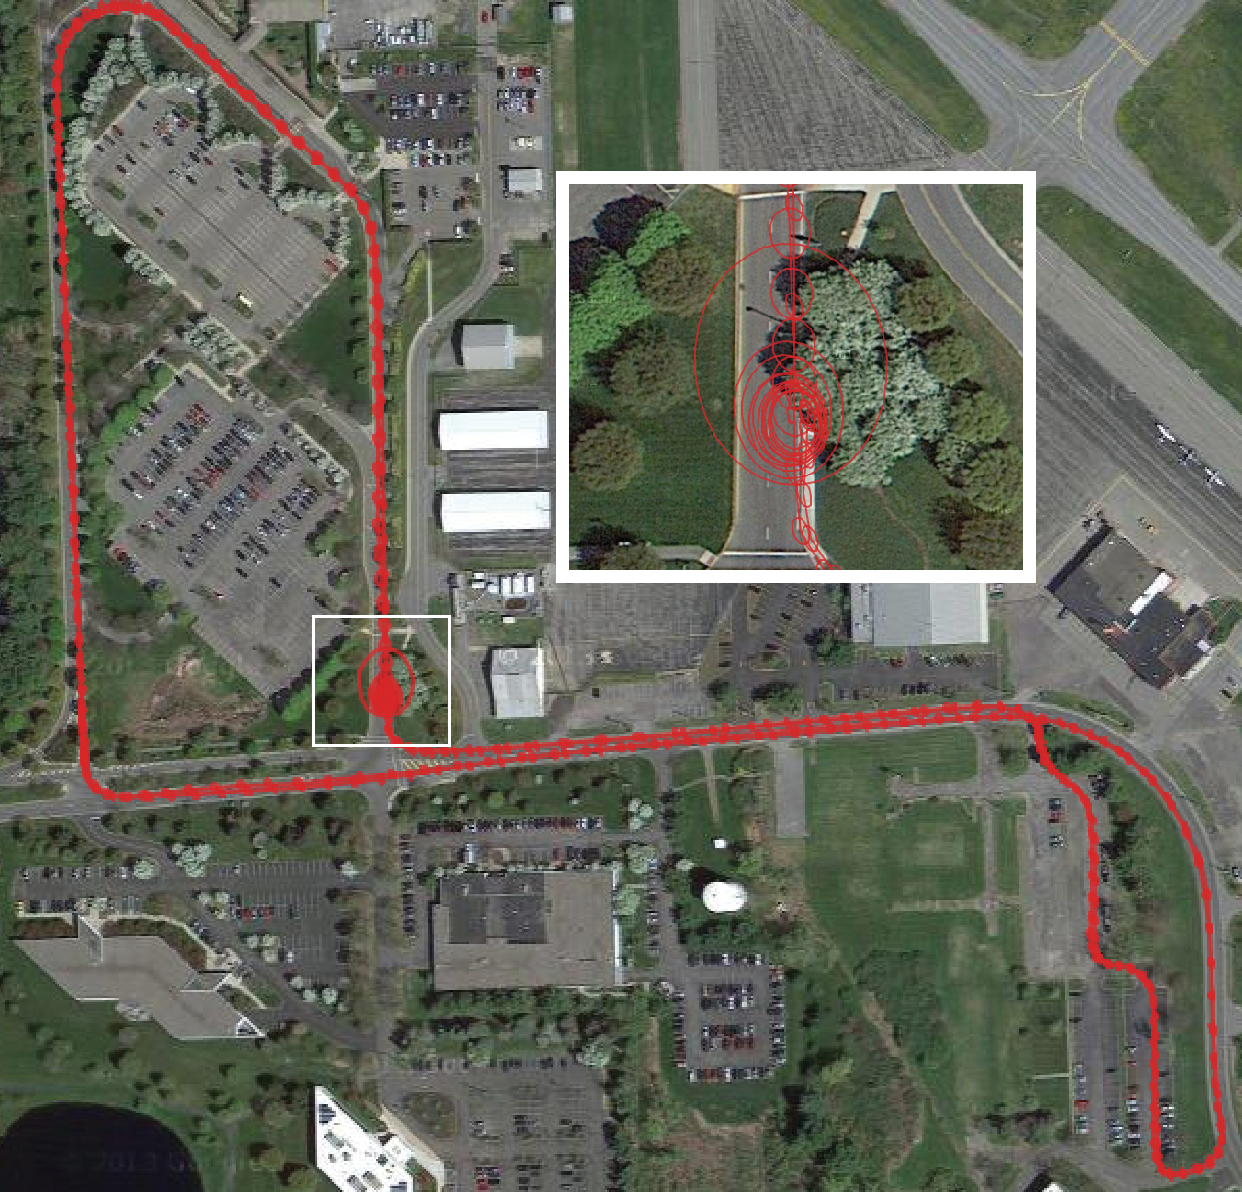
\includegraphics[width=\columnwidth]{airportloop_map}
\caption{Estimated trajectory for \texttt{airportloop} using time-varying Kalman filter adjusted to pass consistency test.  Inset: Initial convergence of estimator at the beginning of the sequence.}
\label{fig:airportloop_map}
\end{figure} 

\begin{figure}
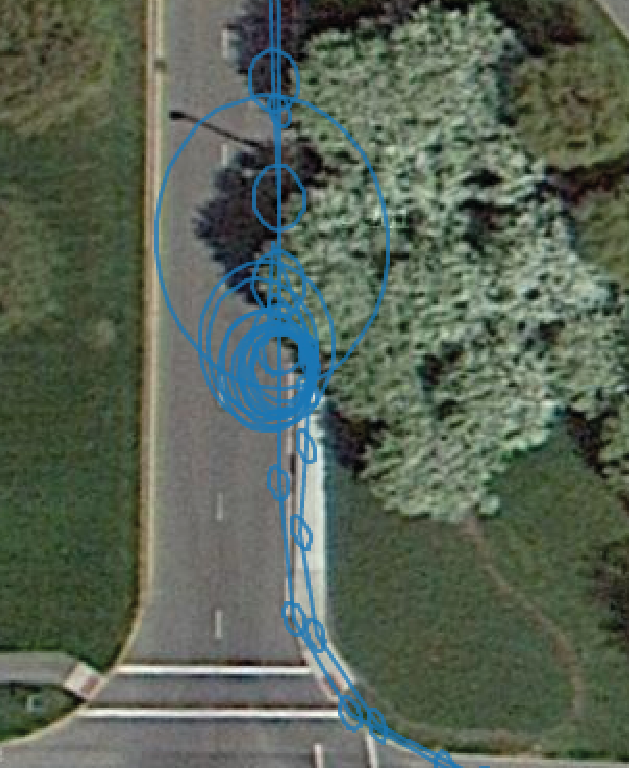
\includegraphics[width=\columnwidth]{airportloop_map_bad}
\caption{Without ensuring filter consistency, the filter can grow over-confident and Kalman filter assumptions that lead to optimality can be broken.  Left: The vehicle is estimated to be on the sidewalk with high confidence.  Right: The original navigation solution is highly erroneous.}
\label{fig:airportloop_map_bad}
\end{figure}

Figure~\ref{fig:nis} shows how the normalized innovations squared statistic, $t_k$ changes over time.  The green lines indicate the test bounds for a 99\% confidence interval and the blue line indicates the test value.  There is a very narrow range for this test to succeed and the trend of the points indicates that even though we successfully found model parameters that helped pass this test, in real world online scenarios, it would be very difficult to do so as subwindows of this data produce different statistics.  This suggestes that our model does not match the system exactly.

\begin{figure}[!b]
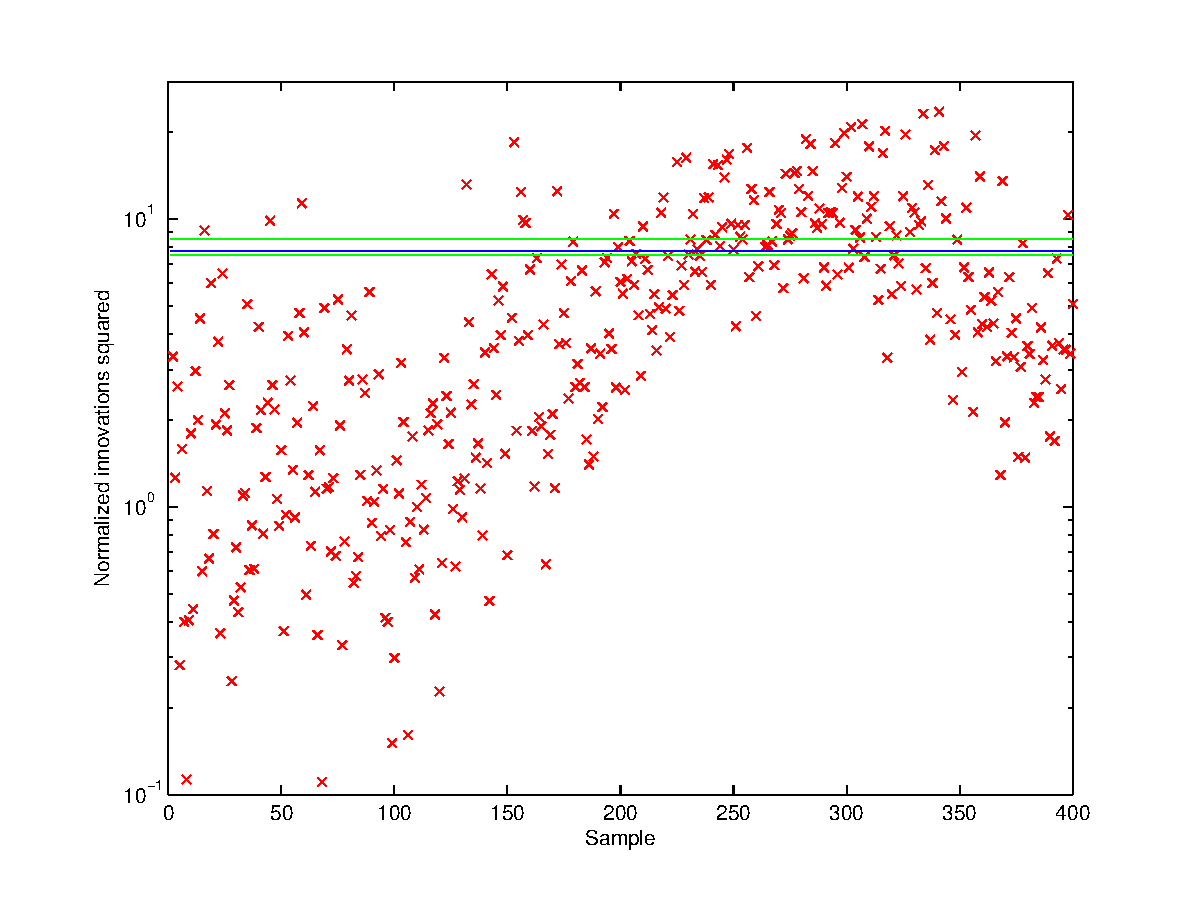
\includegraphics[width=\columnwidth]{nis}
\caption{Normalized innovation squared values for the \texttt{airportloop} dataset.  The green lines represent the test bounds and the blue line is the test statistic.}
\label{fig:nis}
\end{figure}

Since our time-varying Kalman filter propagates an error covariance matrix through the track, we can also evaluate its performance when there is an outage.  Rather than skip missing observations entirely, we perform the prediction step and propagate the a priori state estimate forward.  If we skipped the missing entries entirely, then the estimate's covariance matrix would not adequately grow to accomidate any mismatch between the process and the model.  It also improves the numerical integration of the vehicle's trajectory.  Figure~\ref{fig:outage} shows one such outage.  GPS measurements are disabled for 5 seconds.  The process covariance matrix was tuned down to $Q = 0.1I$ to improve visualization.

\begin{figure}[!t]
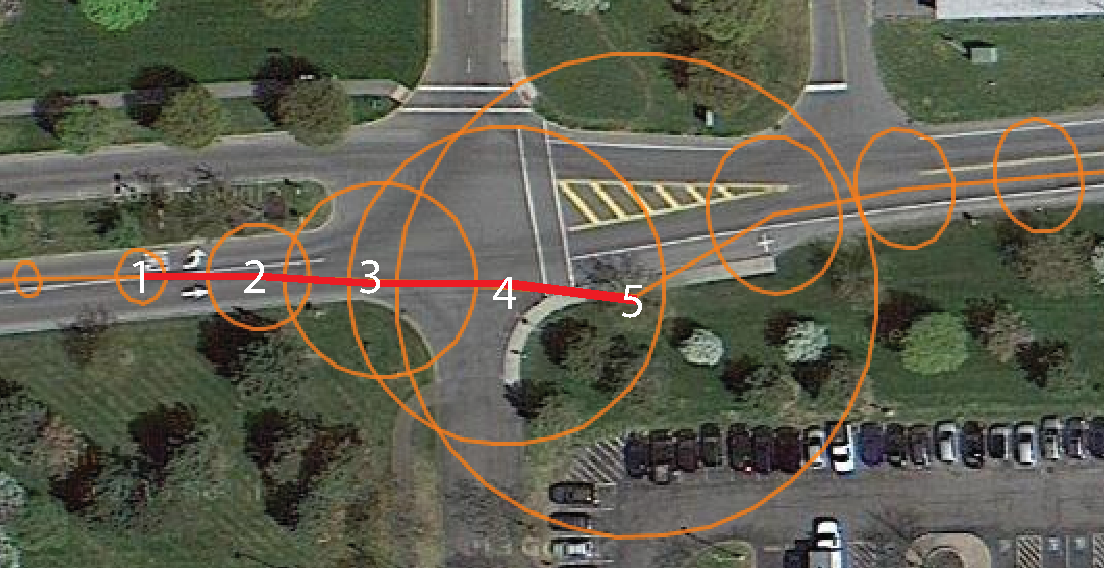
\includegraphics[width=\columnwidth]{outage}
\caption{An artificial 5 second outage during the \texttt{airportloop} dataset.  A priori state estimates during outage marked 1-5.}
\label{fig:outage}
\end{figure}

This dataset did not exhibit any measurements with a large degree of corruption, so we artifically introduced zero-mean Gaussian noise to the pseudorange measurements for satellite 11 for the same 5 second interval as our outage experiment.  If our online consistency hypothesis test can correctly identify erroneous measurements, then the recovery should look exactly like if we did not make those measurements at all.  Figure~\ref{fig:corruption} shows the divergence between the correct trajectory and the measurement-corrupted trajectory.  It also shows the normalized innovation squared measurements exhibit a large increase during this window.  We were unable to find a reliable way to apply the hypothesis test to automatically detect these outliers since the windowed normalized innovation squared statistic varies over time even without measurement corruption.

\begin{figure}[!b]
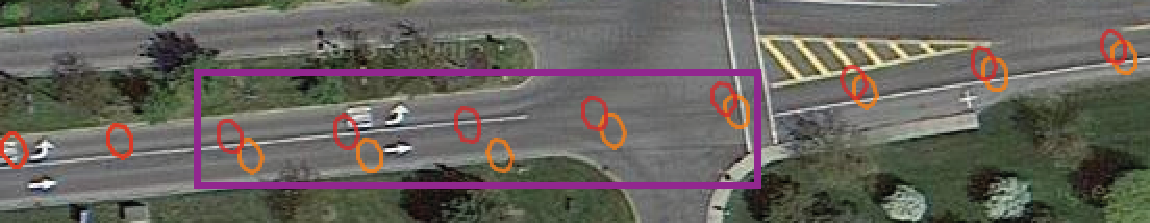
\includegraphics[width=\columnwidth]{corruption}\\
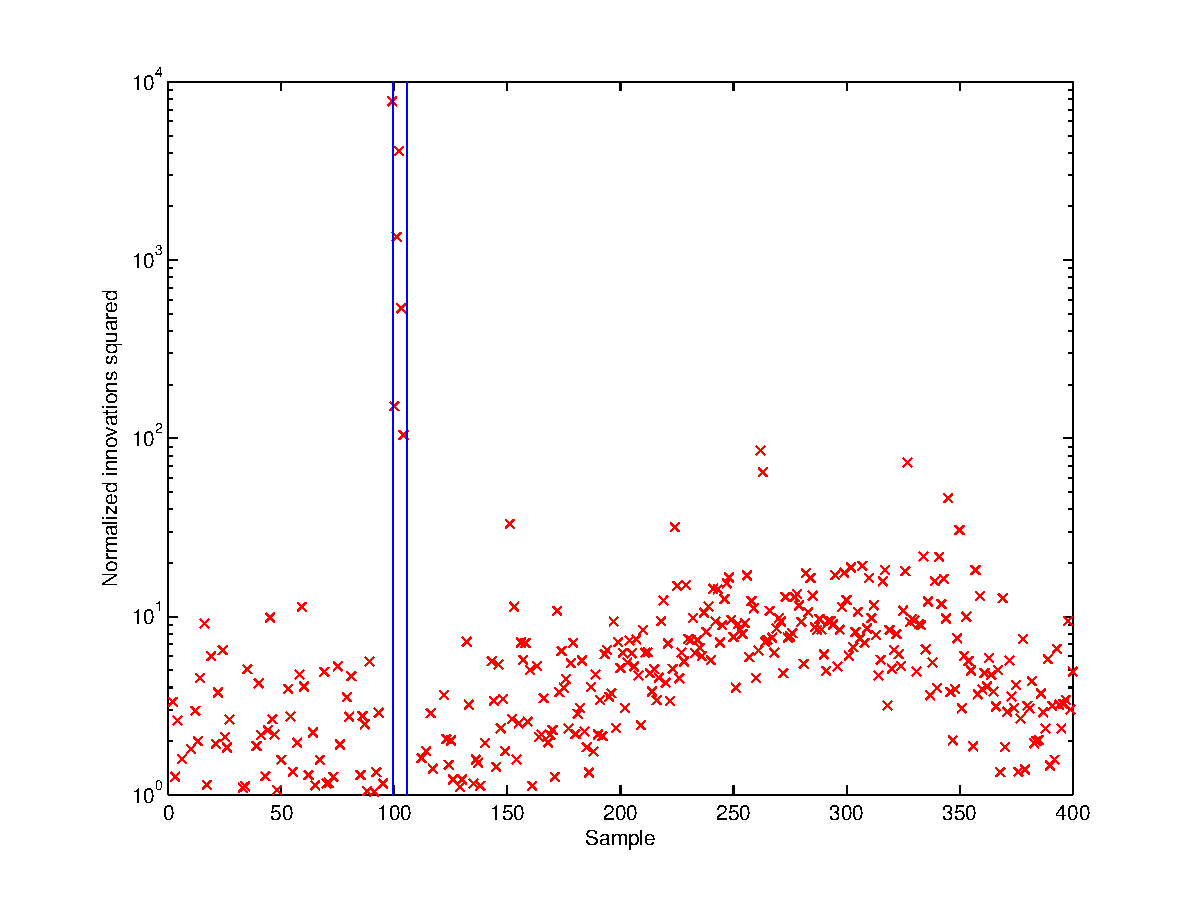
\includegraphics[width=\columnwidth]{nis_corruption}
\caption{Top: Original trajectory in red with corrupted trajectory in orange.  Trajectory is corrupted by introducing zero-mean Gaussian noise to one satellite's pseudorange measurements for 5 seconds, indicated by the violet rectangle.  Bottom: Normalized innovation squared for this sequence.  Blue bars indicate the corruption range.}
\label{fig:corruption}
\end{figure}

\subsection{cudtrt13triphammercu Dataset}
This dataset contains examples of significant drift if velocity is simply integrated.  Figure~\ref{fig:track2_map} shows the different between the time-varying Kalman-filtered track and the integrated track.

\begin{figure}[!b]
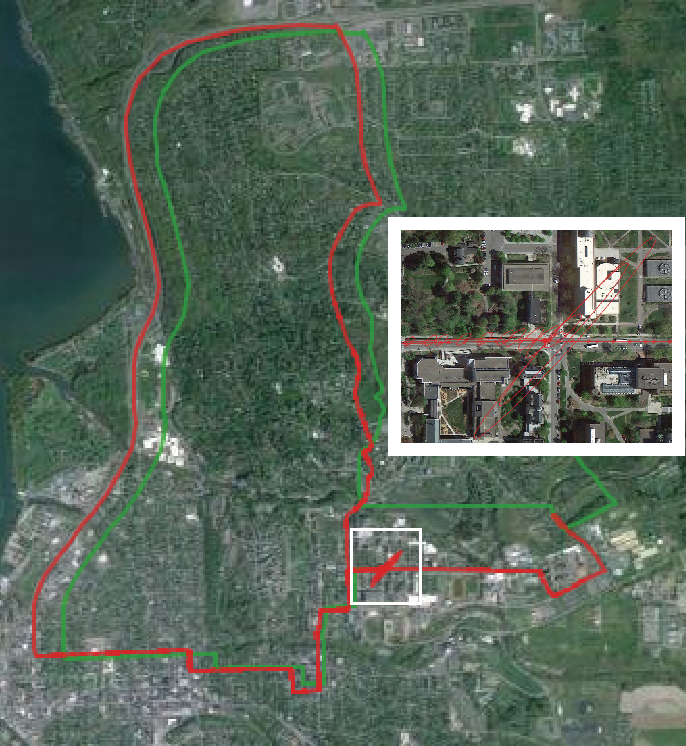
\includegraphics[width=\columnwidth]{track2_map}
\caption{Estimated trajectory for \texttt{cudtrt13triphammercu} dataset using time-varying Kalman filter in red.  Integrated velocity shown in green.  Integrated velocity alone suffers from significant drift.  Inset: Erroneous measurements cause distribution covariance to increase significantly.}
\label{fig:track2_map}
\end{figure}

We artificially introduced the same corruption as for the \texttt{airportloop} dataset, but with a different satellite for 5 seconds on the \texttt{cudtrt13triphammercu}.  The normalized innovation squared values are more consistent in this dataset, so we were able to successfully detect 4 out of 5 corrupt measurements and discard them accordingly.  Figure~\ref{fig:cu_corruption} illustrates how the two trajectories diverge.

\begin{figure}
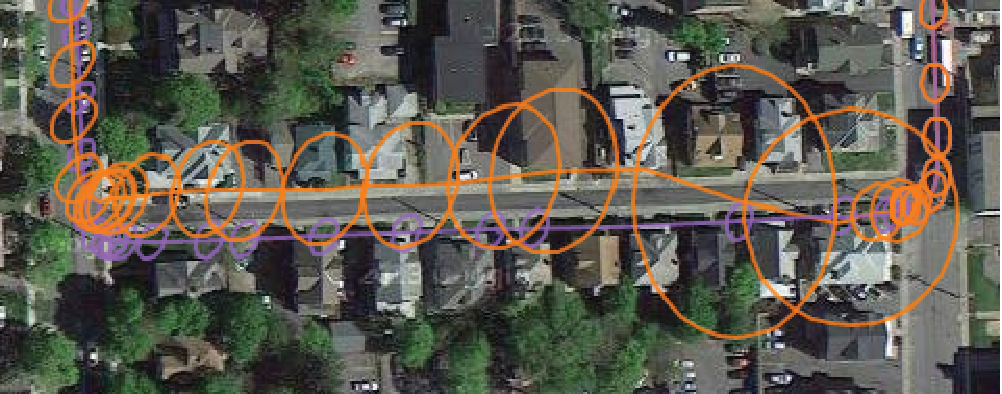
\includegraphics[width=\columnwidth]{cu_corruption}\\
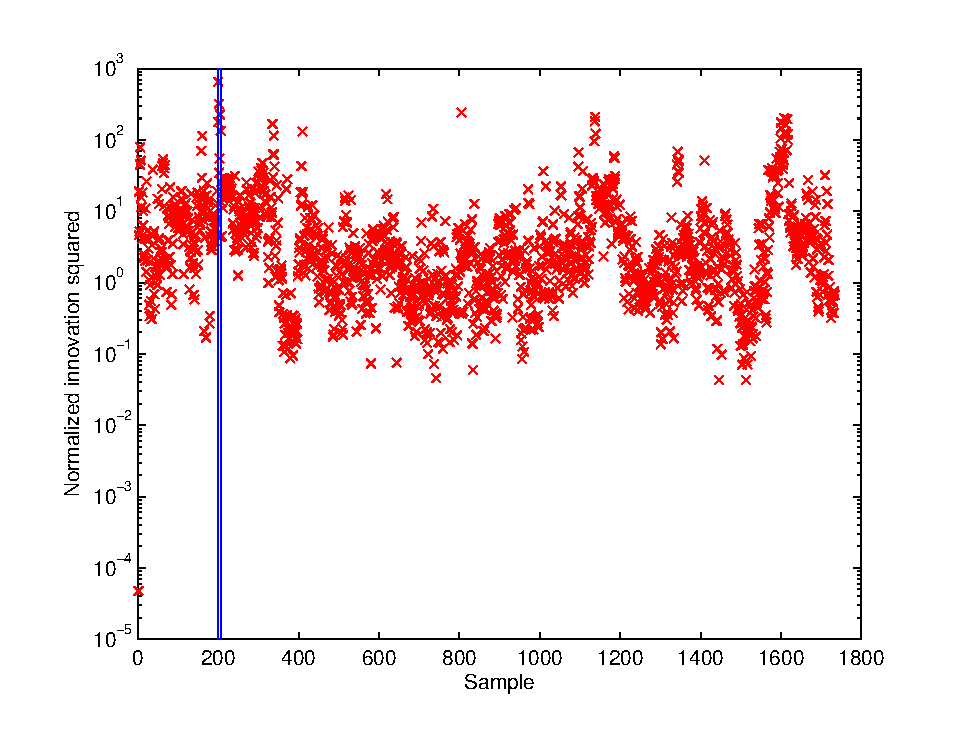
\includegraphics[width=\columnwidth]{nis_cu_corruption}
\caption{Top: The orange estimates are generated by applying the online consistency test to detect faulty measurements while the pink curve becomes biased.  Bottom: The normalized innovation squared values are consistent over time making detection of faulty measurements easy.}
\label{fig:cu_corruption}
\end{figure}

Figure~\ref{fig:max_eigenvalue} shows that for the \texttt{cudtrt13triphammercu} dataset, all eigenvalues are within the unit circle, ensuring a stable filter at each sample time.

\begin{figure}[!t]
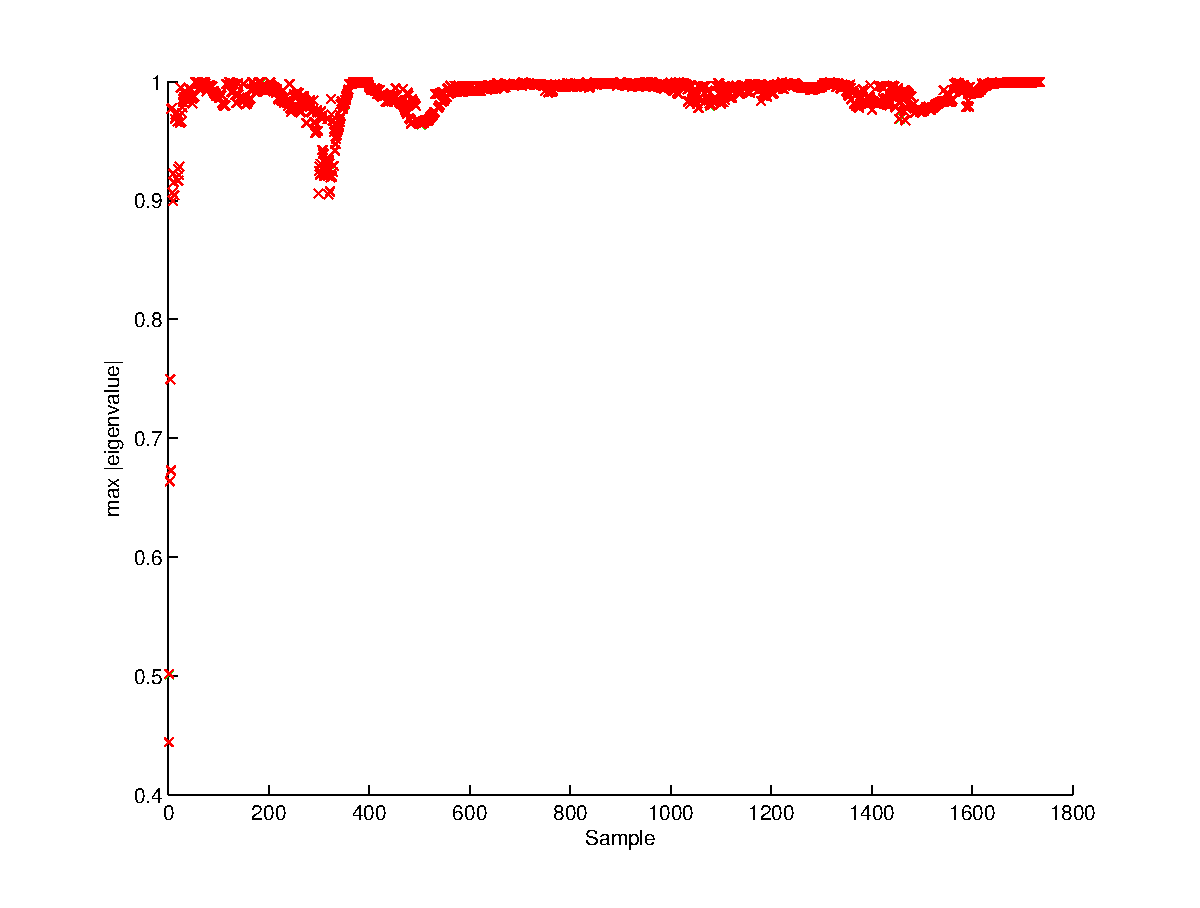
\includegraphics[width=\columnwidth]{eigenvalues}
\caption{Maximum absolute eigenvalues of the closed-loop error dynamics state transition matrix for time-varying Kalman filter on \texttt{cudtrt13triphammercu} dataset.}
\label{fig:max_eigenvalue}
\end{figure}


\section{Conclusion}\label{sec:conclusion}
In this paper we presented several statistics to help tune and validate the design of a Kalman filter for GPS-based localization.  We also proposed an extended model that considered per-satellite biases as part of the estimated state.

Several statistical hypothesis tests were very useful in the design of the filter.  For example, the normalized innovation squared normality test was extremely useful as it allowed us to rapidly scale covariance matrices on a per dataset basis.  The primary drawback is that since we had a model mismatch, it was very difficult to tune the system to achieve success on the test.  Figure~\ref{fig:nis} shows that the acceptable bad is extremely small for a 99\% confidence interval given that the normalized innovation squared values have such high variance and that the normalized innovation squared values undergo a change throughout the experiment.  However, Figure~\ref{fig:nis_stationary} shows that for a stationary receiver, the assumptions match quite well.  The smooth trends in these normalized innovation squared plots indicate that it might be beneficial to explore more dynamic forms of the process and measurement noise covariance matrices.  An attempt was made to dynamically scale $\alpha_k$ for the process covariance, but it was difficult to prevent the system from going unstable.  Since scaling the measurement covariance matrix offered the ability to pass the global consistency tests, then perhaps more focus should be placed on automatically scaling this matrix under the assumption that $\sigma_{PR}$ and $\sigma_D$ and poorly estimated as-is.

The Ljung-Box test for multivariate independence was not very useful.  All of the data used in the experiments intuitively had correlations and the statistical hypothesis test reflected that.  As explored in lab, it's possible to find an appropriate lag at which measurements are no longer correlated, but for a mobile receiver, it's probably the case that it's safer to break the independence assumption rather than only take one sample every 50 seconds.  Despite violating the independence assumptions, the filter qualitatively performed quite well localizing the vehicle in the driving corridor despite largely erroneous navigation solutions.

It's unclear whether the bias-adjusted time-varying Kalman filter formulation was a step in the right direction.  While its impact was validated in terms of reduced position error on the stationary dataset, it also caused the jerk normality test to fail suggesting that an additional systematic bias was introduced into the filter.  For mobile datasets, it offered little difference which is why results were omitted for those datasets in this paper.  A more principled approach to addressing the slowly varying errors in GPS measurements might be to instead use the Extended Kalman filter to model this as a non-linear system, extend the measurements to include raw GPS observables, error correction factors, etc. and track per satellite states in the filter's state vector.  In some sense, this current implementation is nearly using an EKF except all of the non-linear parts have been factored away into \texttt{solveposvelod}.  All of the work done by \texttt{solveposvelod} could instead be hoisted into the Jacobian of the EKF. 


{\small
\bibliographystyle{ieee}
\bibliography{all}
}

\pagebreak
\onecolumngrid
\appendix
\section{Main Filter Code}
\subsection{filter\_dataset.m}
\lstinputlisting[language=Matlab]{filter_dataset.m}
\subsection{process\_matrix.m}
\lstinputlisting[language=Matlab]{process_matrix.m}
\subsection{state\_vector.m}
\lstinputlisting[language=Matlab]{state_vector.m}
\subsection{create\_state.m}
\lstinputlisting[language=Matlab]{create_state.m}
\subsection{solveposvelod\_DOP.m}
\lstinputlisting[language=Matlab]{solveposvelod_DOP.m}
\subsection{feedback.m}
\lstinputlisting[language=Matlab]{feedback.m}
\subsection{measurement\_covariance.m}
\lstinputlisting[language=Matlab]{measurement_covariance.m}
\subsection{measurement\_vector.m}
\lstinputlisting[language=Matlab]{measurement_vector.m}

\section{Filter Gain Code}
\subsection{gain\_factory.m}
\lstinputlisting[language=Matlab]{gain_factory.m}
\subsection{static\_slow\_gain.m}
\lstinputlisting[language=Matlab]{static_slow_gain.m}
\subsection{static\_fast\_gain.m}
\lstinputlisting[language=Matlab]{static_fast_gain.m}
\subsection{kalman\_steady\_state\_gain.m}
\lstinputlisting[language=Matlab]{kalman_steady_state_gain.m}
\subsection{kalman\_time\_varying\_gain.m}
\lstinputlisting[language=Matlab]{kalman_time_varying_gain.m}

\section{Dataset Management Code}
\subsection{load\_dataset.m}
\lstinputlisting[language=Matlab]{load_dataset.m}
\subsection{visible\_satellite\_filter.m}
\lstinputlisting[language=Matlab]{visible_satellite_filter.m}
\subsection{format\_doppler\_shift.m}
\lstinputlisting[language=Matlab]{format_doppler_shift.m}
\subsection{load\_ephem.m}
\lstinputlisting[language=Matlab]{load_ephem.m}
\subsection{load\_weather.m}
\lstinputlisting[language=Matlab]{load_weather.m}

\section{Visualization Code}
\subsection{draw\_trajectory.m}
\lstinputlisting[language=Matlab]{draw_trajectory.m}
\subsection{save\_as\_geojson.m}
\lstinputlisting[language=Matlab]{save_as_geojson.m}

\section{Evaluation Code}
\subsection{compute\_jerk.m}
\lstinputlisting[language=Matlab]{compute_jerk.m}
\subsection{evaluate\_innovation\_whiteness.m}
\lstinputlisting[language=Matlab]{evaluate_innovation_whiteness.m}
\subsection{evaluate\_jerk\_normal.m}
\lstinputlisting[language=Matlab]{evaluate_jerk_normal.m}
\subsection{evaluate\_jerk\_whiteness.m}
\lstinputlisting[language=Matlab]{evaluate_jerk_whiteness.m}
\subsection{max\_abs\_eigenvalues.m}
\lstinputlisting[language=Matlab]{max_abs_eigenvalues.m}
\subsection{nis.m}
\lstinputlisting[language=Matlab]{nis.m}
\subsection{plot\_t.m}
\lstinputlisting[language=Matlab]{plot_t.m}
\subsection{stationary\_rmse.m}
\lstinputlisting[language=Matlab]{stationary_rmse.m}
\subsection{whiteness\_test.m}
\lstinputlisting[language=Matlab]{whiteness_test.m}
\subsection{whiteness\_test\_portmanteau.m}
\lstinputlisting[language=Matlab]{whiteness_test_portmanteau.m}




\end{document}

